\section{Energy Efficient CNFET-based Cache Design} \label{sec:warp}
The energy consumption of accessing '0' and '1' in CNFET-based SRAM cell 
differs dramatically. By taking advantage of the feature, we propose 
an adaptive run-time encoding approach and build an energy efficient 
CNFET-based cache named CNT-Cache. The architecture as well as the 
encoding approach will be detailed in this section.

\begin{figure}
    \center{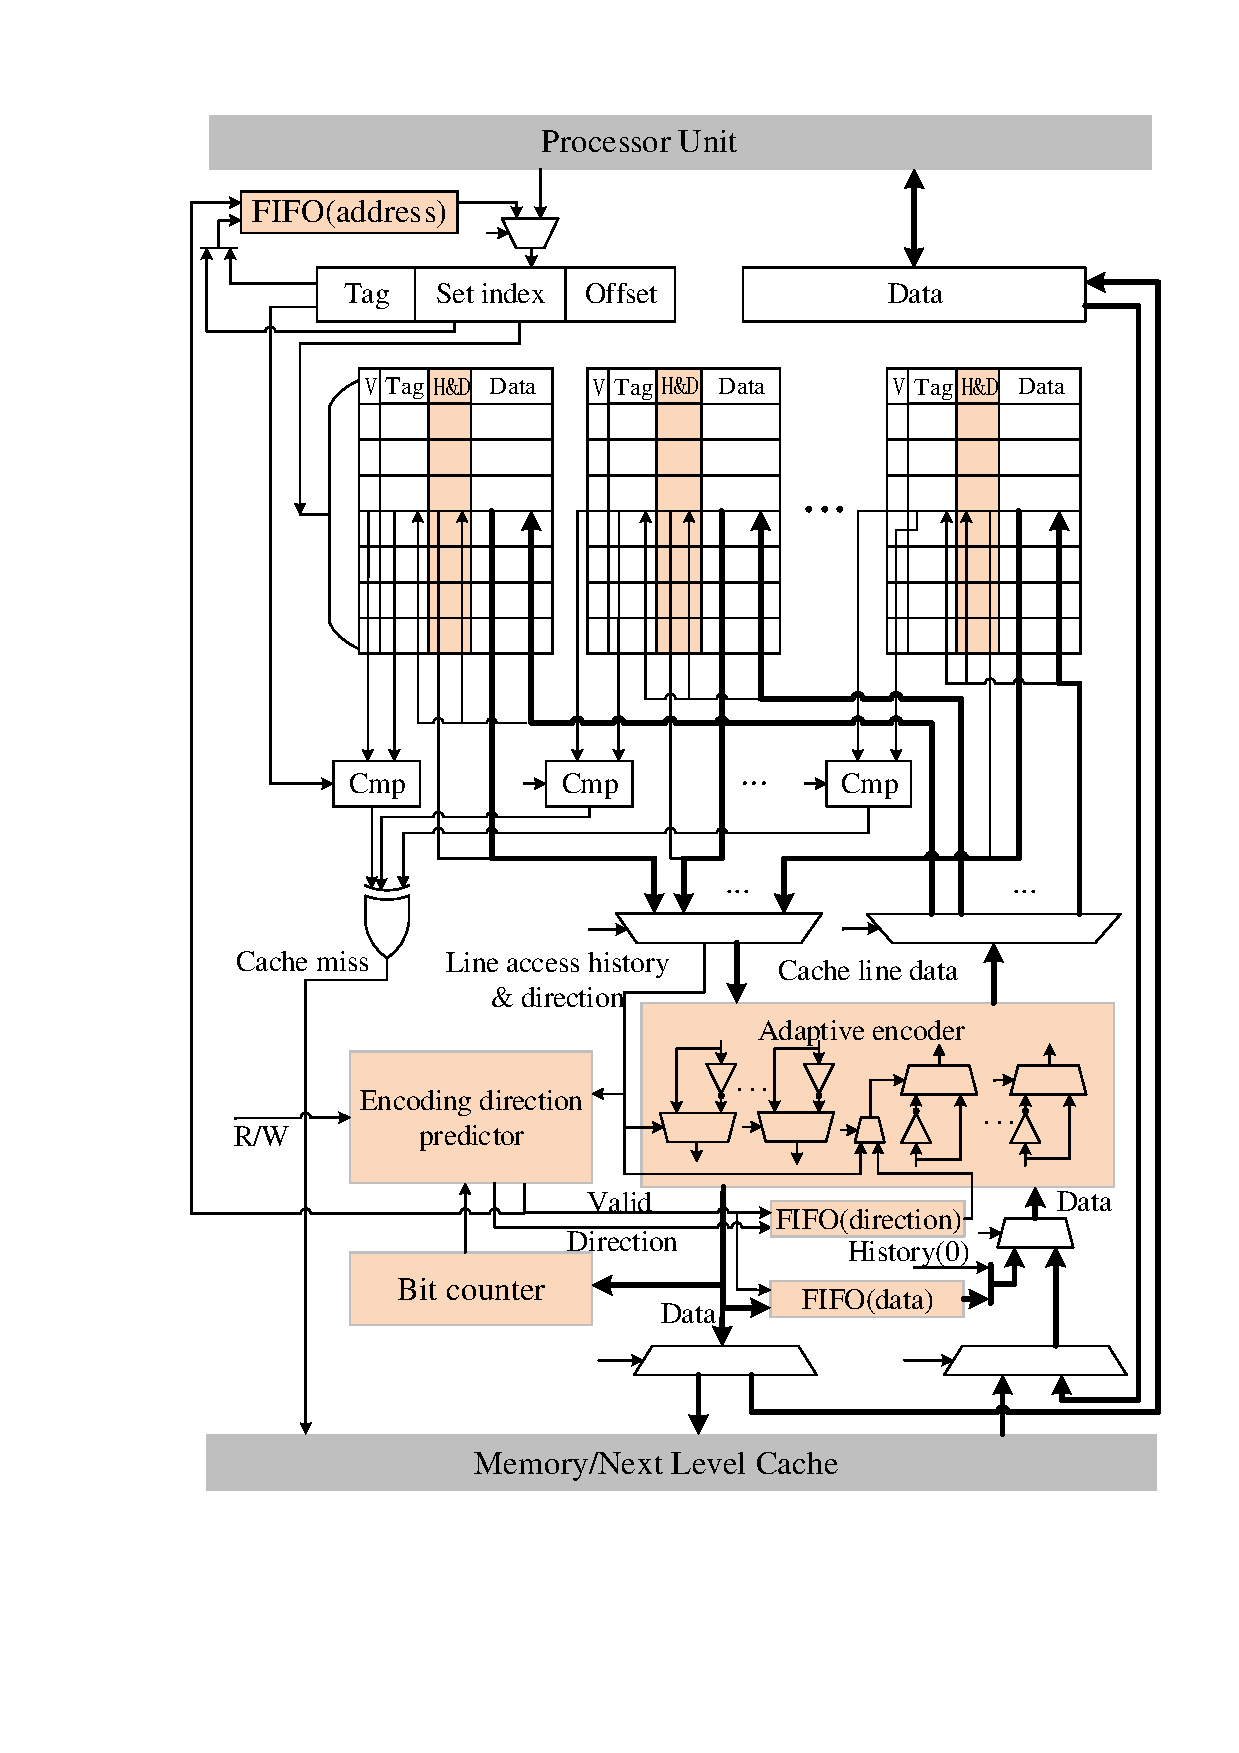
\includegraphics[width=0.88\linewidth]{cache_archi}}
    \caption{Architecture of CNT-Cache}
\label{fig:architecture}
\vspace{-1em}
\end{figure}

\subsection{CNT-Cache Overview}
Figure \ref{fig:architecture} illustrates the proposed CNT-Cache 
architecture with adaptive encoding support.
Compared to a typical cache architecture, it requires a few additional 
components as highlighted in orange. The most critical part is the 
adaptive encoding module. It can encode each cache line data with 
either more '1' bits or '0' bits depending on the cache line operation 
preferences. For example, suppose the original data has more '1' bits and 
the operation is more efficient in handling '0' according 
to Table \ref{tab:rw-analysis}. Then we can encode the 
data by inverting each bits and have an additional bit to record the encoding 
direction. Note that the operation can either be read or write. Meanwhile, 
the adaptive encoder is essentially a series of inverters
with 2-to-1 multiplexers and operates based on the encoding direction bit read from 
each cache line. The simple structure has negligible influence 
on the timing of the critical data path. 

Another key component is the encoding direction predictor. 
It determines the encoding pattern or preference of each cache line based on 
a window of historical accesses. With the access pattern (i.e. the number of read 
and the number of write in a window), it checks whether the current cache 
line data matches the cache line encoding direction.
If the current encoding does not fit the cache line data, we
change the encoding direction and update the cache line data accordingly.
To avoid affecting the cache write data path, a data FIFO is used to delay the update
until there is an idle time slot. Meanwhile, an index FIFO is also needed to 
decide the update cache line address synchronously. Also the cache line history 
will be reset. If there is no need to change the encoding,
we just update the cache access counter in history region in the cache line.
To enable encoding direction prediction of each cache line, we have each 
cache line access history stored along with the cache line data. Therefore, we need to 
widen the cache line to store the access history as well 
as the encoding direction. The added bits are marked as 'H\&D' (history and direction) in Figure \ref{fig:architecture}.

In general, the proposed CNT-Cache adjusts the cache line encoding 
based on the cache line data access pattern to minimize the overall 
cache access energy consumption. The encoding is in the cache 
operation data path, so it must be simple for efficient 
hardware implementation. The predictor determines the cache line 
encoding direction based on the access history in a window as 
well as the encoding switch overhead. It requires more computing 
but will not affect the critical data paths of the cache operations. 

\subsection{Cache line data encoder}
The cache line data encoder operates based on the encoding direction 
read from the corresponding cache line. When there are less 
preferred bits in the cache line data, typically we need to invert 
the whole cache line. Nevertheless,
this approach may fail to explore the continuous preferred bits 
in the data and convert them to bits that are inefficient for 
the cache operations. To address this problem, we adopt a fine-grained 
encoding approach to further reduce the inefficient bits in the data. 
Basically the input data is divided into multiple partitions and 
each partition is encoded independently to maximize the preferred bits.
In this case, % each partition needs one bit to record the encoding direction and 
we need to add more direction bits to each cache line.

To help illustrate the partitioned encoding, an example is presented in 
Figure \ref{fig:encode}. The raw data has much more '0' bits than '1' bits.
When the cache line is read intensive, %according to the encoding direction, 
the data needs to be inverted using the baseline encoding approach. 
In this case, the $(K-1)$th partition of the cache line data with more '1' bits 
are inverted though they are preferred for cache read. 
When the partitioned encoding approach is applied, the $(K-1)$th 
partition remains unchanged. Similar optimization opportunities can also be explored 
when the cache line is write intensive. Compared to the baseline encoding,
the partitioned encoding needs more direction bits.

\begin{figure}
    \center {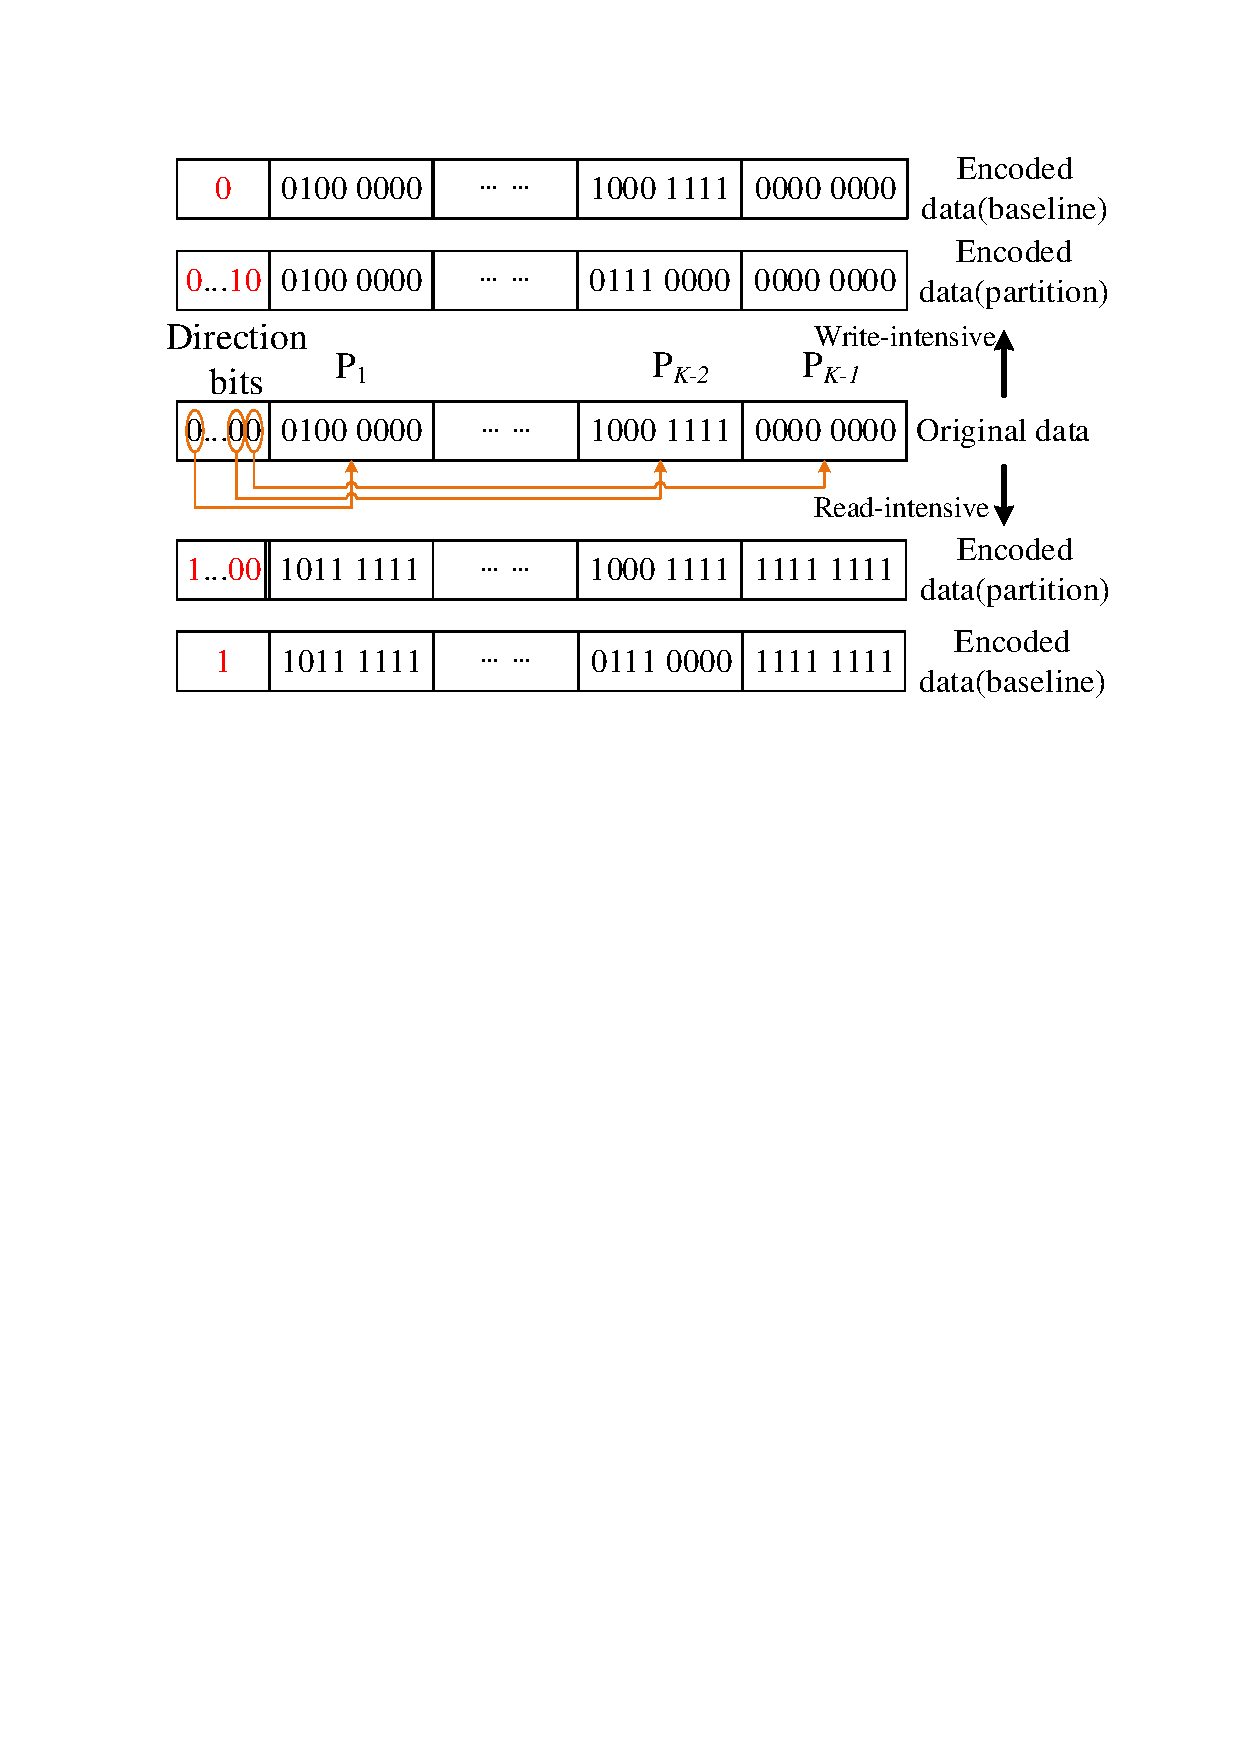
\includegraphics[width=0.85\linewidth]{encode}}
    \caption{An example of partitioned cache line encoding}
\label{fig:encode}
\vspace{-1em}
\end{figure}

The adaptive encoding module is essentially a series of inverters and 2 to 1 multiplexers
as described in Figure \ref{fig:architecture}.
When the partitioned encoding approach is utilized, the select signal of the multiplexers 
that are originally shared by the whole cache line data are now replaced with the partition 
direction bits instead. It has little influence on timing of the encoder module design. 

\subsection{Encoding direction predictor}
Encoding direction predictor determines the encoding of each cache line data.
It is of vital importance to the energy efficiency of the CNT-Cache.
While achieving optimal encoding for each cache access may cause frequent encoding 
direction switch and the switch overhead is non-trivial, thus the predictor 
performs prediction in the granularity of a window of accesses and decides if the encoding 
should be updated.

The proposed prediction strategy can be roughly divided into two steps as 
shown in Algorithm \ref{alg:prediction}. Firstly, we mainly analyze the operation 
preference of the cache line based on the access history. 
Basically, we keep a window $W$ of the latest accesses. 
$W$ also represents the prediction cycle. Within $W$, 
if the number of read is larger than a threshold $Th_{rd}$, 
it indicates that the cache line is read intensive. 
Otherwise, it is considered to be write intensive. 
The threshold is used to determine if it saves energy 
when we encode the stored data for reading. 
Suppose there are $x$ '0' bits and $y$ '1' bits on 
average in a window of accesses. Without loss of generality, assume $x<y$. 
The energy consumption using different encoding can be calculated with 
Equation \ref{eq:read_encoding_energy} and Equation \ref{eq:write_encoding_energy} 
respectively. Here $E_{rd0}$, $E_{rd1}$, $E_{wr0}$ and $E_{wr1}$ refer to 
the energy consumption of reading bit'0'/'1' and writing bit'0'/'1'. When $E_{rd\_enc}$ and $E_{wr\_enc}$ is equal, we can obtain $Th_{rd}$ using Equation \ref{eq:threshold}. 
Since $E_{rd0} - E_{rd1}$ is quite close to $E_{wr1} - E_{wr0}$ 
according to Table \ref{tab:rw-analysis}, $Th_{rd}$ is roughly half of $W$.

\begin{algorithm}
    \renewcommand{\algorithmicrequire}{\textbf{Input:}}
	\renewcommand{\algorithmicensure}{\textbf{Output:}}
    \caption{Encoding direction prediction algorithm} 
    \label{alg:prediction}
    \footnotesize
	\begin{algorithmic}[1] 
	    \REQUIRE Cache line access history including access 
	    number $A_{num}$, the number of write accesses $Wr_{num}$, and 
	    maximum access per prediction $W$, Cache line encoding direction $D$, 
	    Read intensive threshold $Th_{rd}$, Cache line data $Data$, 
	    Bit '1' number threshold array for encoding switch $Th_{bit1num}[W]$.
	    
	    \ENSURE Cache line access pattern ${Pattern}$, new encoding direction $D_{new}$ and 
	    new encoded data $Data_{new}$.
	    
	    \IF{($A_{num} = W$)}
	        \STATE
	        \STATE // Step 1: access pattern prediction
	        \IF{($Wr_{num} > Th_{rd}$)}
	            \STATE $Pattern \gets 1$ // write intensive
	        \ELSE
	            \STATE $Pattern \gets 0$ // read intensive
	        \ENDIF

            \STATE
            \STATE // Step 2: check if the cache line encoding will be changed.
	        \STATE $bit1num \gets getNumOfBit1(Data)$ // count '1' in $Data$
	        \IF {($Pattern = 1$)} %// write intensive
	            \IF{($bit1num > Th_{bit1num}[Wr_{num}]$)}
	                \STATE $D_{new} \gets \lnot D$
	                \STATE $Data_{new} \gets \lnot Data$
	            \ENDIF
	       \ELSE
	            \IF{($bit1num < Th_{bit1num}[Wr_{num}]$)}
	                \STATE $D_{new} \gets \lnot D$
	                \STATE $Data_{new} \gets \lnot Data$
	            \ENDIF
	       \ENDIF
	       
	       \STATE $A_{num} \gets 0$
	       \STATE $Wr_{num} \gets 0$
	       
	    \ELSE
	    	\STATE $Wr_{num} \gets Wr_{num} + 1$ when there is a cache write.
	        \STATE $A_{num} \gets A_{num} + 1$ when there is a cache access.
	    \ENDIF
	 
	%\EndProcedure
	\end{algorithmic}
\end{algorithm}

\footnotesize
\begin{equation}
    \label{eq:read_encoding_energy}
    \begin{split}
    E_{rd\_enc}=Th_{rd} \times (x \times E_{rd0} + y \times E_{rd1}) + \\ (W - Th_{rd}) \times (x \times E_{wr0} + y \times E_{wr1}) \\
    \end{split}
\end{equation}

\begin{equation}
    \label{eq:write_encoding_energy}
    \begin{split}
    E_{wr\_enc}=Th_{rd} \times (y \times E_{rd0} + x \times E_{rd1}) + \\ (W - Th_{rd}) \times (y \times E_{wr0} + x \times E_{wr1}) \\
    \end{split}
\end{equation}

\begin{equation}
\label{eq:threshold}
    \begin{split}
    % E_{rd\_enc} - E_{wr\_enc} = (y-x)(Th_{R/W} \times (E_{rd0} - E_{rd1}) + \\  (W-Th_{R/W}) \times (E_{wr0} - E_{wr1})) = 0 \\
    Th_{rd} = W \times \frac{1}{1 + \frac{E_{rd0} - E{rd1}}{E_{wr1}-E_{wr0}}}
    \end{split}
\end{equation}
\normalsize

As we predict the cache line read/write preferences using the two access 
counters i.e. $A_{num}$ and $Wr_{num}$, we need $2\times log{2}{W}$ 
bits to store them in each cache line. While it is usually expensive 
to add bits to the cache line, $W$ must be set properly to 
reduce the overhead of history bits.

In the second step, we mainly evaluate the current cache line data
and see if it fits the encoding and the access preferences in history, 
which is already determined in the first step. An intuitive approach 
is to calculate the energy efficiency of operating on the cache line 
data and compare with the cache access energy efficiency using a 
different encoding. If it consumes less energy, it means that the cache 
line data encoding is optimal. Otherwise, we need to reset the encoding 
and update the data stored in the cache line. 

The energy consumption of current cache line data access $E$ can be 
calculated using Equation \ref{eq:energy-efficiency}.
When a different encoding approach is used, the energy consumption 
becomes $\bar{E}$ as given in Equation \ref{eq:_energy-efficiency}.
Suppose $E_{encode}=N_{1} \times E_{wr0} + (L - N_{1}) \times E_{wr1}$ stands for the energy consumption of a cache 
line encoding switch which essentially updates the re-encoded data to cache.
When $E = \bar{E} + E_{encode}$, we can obtain the bit number ('1') threshold 
$Th_{bit1num}$ as presented in Equation \ref{eq:bit1num} 
where $E_{save} = (W-Wr_{num}) \times (E_{rd0}-E_{rd1}) - Wr_{num}\times(E_{wr1}-E_{wr0})$. 
Note that $bit1num$ represents the number of '1' bits in the data. 
It can be calculated using a bit counting function $getNumOfBit1()$ as described in 
Algorithm \ref{alg:prediction}. To make the representation short, 
we set $N_{1} = bit1num$. $L$ is the cache line length.

According to Equation \ref{eq:bit1num}, the threshold also depends on 
the cache line access history i.e. $Wr_{num}$ and it needs to be calculated at run-time.
Fortunately, we can obtain all the possible bit number threshold in advance 
and construct an array $Th_{bit1num}$ as presented in Algorithm \ref{alg:prediction}. 
The array can be implemented with a table that has $W$ entries. 
It returns the exact bit number threshold given $Wr_{num}$. In this case, the predictor 
can compare the number of bit '1' in the cache line with the threshold read from the 
table, and decides if it is necessary to inverse the encoding rapidly, which greatly 
simplifies the predictor design. 

\footnotesize
\begin{equation}
    \label{eq:energy-efficiency}
    \begin{split}
        %E=(W-Wr_{num}) \times (bit1num \times E_{rd1} + (L - bit1num) \times E_{rd0}) + \\
        %Wr_{num} \times (bit1num \times E_{wt1} + (L - bit1num) \times E_{wt0})
        E=(W-Wr_{num}) \times (N_{1} \times E_{rd1} + (L - N1) \times E_{rd0})\\
        + Wr_{num} \times (N_{1} \times E_{wr1} + (L - N1) \times E_{wr0})
    \end{split}
\end{equation}

\begin{equation}
    \label{eq:_energy-efficiency}
    \begin{split}
        %\bar{E}=(W-Wr_{num}) \times (bit1num \times E_{rd0} + (L - bit1num) \times E_{rd1}) + \\
        %Wr_{num} \times (bit1num \times E_{wt0} + (L - bit1num) \times E_{wt1})
        \bar{E}=(W-Wr_{num}) \times (N_{1} \times E_{rd0} + (L - N_{1}) \times E_{rd1}) \\ 
        + Wr_{num} \times (N_{1} \times E_{wr0} + (L - N_{1}) \times E_{wr1})
    \end{split}
\end{equation}

%\begin{equation}
%    \label{eq:energyencoding}
%    \begin{split}
%        E_{encode}=N_{1} \times E_{wr0} + (L - N_{1}) \times E_{wr1}
%    \end{split}
%\end{equation}

%\begin{equation}
%    \label{eq:save}
%        E_{save} = (W-Wr_{num}) \times (E_{rd0}-E_{rd1}) - Wr_{num}\times(E_{wr1}-E_{wr0})
%\end{equation}

\begin{equation}
    \label{eq:bit1num}
    \begin{split}
        N_{1} = \frac{L \times (E_{save} - E_{wr1})}{2\times E_{save} - (E_{wr1}-E_{wr0})}
    \end{split}
\end{equation}
\normalsize

%In addition, how to determine the data encoding pattern of the current cache block is the key to the effect of the above run-time encoding strategy. Because the misjudgment of each data encoding pattern will cause incorrect data encoding and sub-optimal performance.The sub-optimal performance can offset the overall optimization effect of the entire CNT-cache evenly. There are two things need to be considered when developing a effective judgment model: Firstly, the data encoding pattern of cache block should be determined by its previous access mode rather than recent access mode. Simply encoding data with its most recent access mode may result in frequent switching between different optimization patterns, which will cause energy waste. Secondly, the encoding phase should be removed from the critical path. For example, if every normal access to the cache needs to wait for the results of the prediction process, the delay it generates will significantly affect the performance of the cache.

%In general, the dynamic power consumption of cache in a period of time can be calculated by using the following formula:
%\begin{align}
%E = N_{allr} \times E_{avgr} + N_{allw} \times E_{avgw}
%\end{align}
%where, $N_{allr}$ and $N_{allw}$indicates the overall number of read- /write- accesses to the cache during run-time.$E_{avgr}$ and $E_{avg_w}$ represent the average read or write power consumption for a cache block. 
%However, in this article, not only how many cache blocks are read/written, but also the 0/1 number of stored data should be considered. So the above formula can be written as:
%\begin{align}
%E = \sum_{C=0}^N(E_{cache block})
%\end{align}
%\begin{align}
%E_{cache block} = E_{read} \times N_{read} + E_{write} \times N_{write}
%\end{align}
%\begin{align}
%E_{read} = N_{read0} \times E_{read0} + N_{read1} \times E_{read1}
%\end{align}
%\begin{align}
%E_{write} = N_{write0} \times E_{write0} + N_{write1} \times E_{write1}
%\end{align}
%Here $E_{cache block}$, $E_{read}$ and $E_{write}$ indicates the power consumption of one single cache block or one single read-/write to a cache block, $N_{read}$ and $N_{write}$ represents the number of read/write accesses to the cache block in a period if time. C and N are used to summarize the dynamic power consumption of all cache blocks during the period of time.

%Then, during the run-time of the system, we divide the run-time into small segments for each cache block(checkpoint), And record the number of accesses and write accesses to the current cache line during the checkpoint($AC$ indicates whether a checkpoint is completed and $WC$ indicates the number of write accesses). After that, the number of bit 0/1 in stored data will be recorded by Bit Counter, and the dynamic power consumption of each optimization direction will be calculated and compared. Finally, if the new direction performs better, the data encoding and write back processes will be started, updating the flag bits and real data while clearing other flag information. one thing to note here is that if the encoding direction changes, it will cause an additional writeback operation, so here a write operation is added when calculating the dynamic power consumption of the new direction, which means $E_{new} = E_{read} \times N_{read} + E_{write} \times (N_{write} + 1)$.

%Of course, it is unrealistic to calculated the above formula for each pattern prediction, because the formula above is too complicated. It is found that the TB(defined as the threshold for the number of Bits 1 when the mode changes) is related to the number of write accesses and k via calculation Within a limited number of accesses. Once these three values are determined, the TB is uniquely determined. Since the size of checkpoint and K are pre-set, only a small hash table(equal to the size of checkpoint) is needed to avoid all calculations.
	

%\subsubsection{Threshold}
%As mentioned above, firstly, the access power consumption can be reduced only by accurately predicting the access pattern of each cache block, because inaccurate access pattern prediction will only lead to higher waste of access energy. Secondly, the optimization type of the cache block should be determined by its previous access pattern, since simply encoding the data with the latest access mode may result in frequent switching between different optimization methods, which will cause additional energy wastage. In order to avoid inaccurate data encoding as much as possible, we introduce a threshold $\Delta$T to determine whether the optimization pattern of current cache block needs to be changed. The $\Delta$T indicates that the new encoding direction saves more than $\Delta$T of the original one during the checkpoint. In other words, the new pattern becomes the stable optimization pattern only when $E_{original} - E_{new} > \Delta T \times E_{original}$ is satisfied. In summary, the algorithm of the pattern predictor is shown in Algorithm.\ref{alg:prediction}. By default, we set checkpoint as 15 accesses operation to each cache block. And in order to save the maximum power overhead, we will explore the relationship between $\Delta$T and dynamic energy saving through a series of experiments. The results are shown in section\ref{sec:result}.
